In this appendix we will illustrate basic mathematical tools used all through the thesis.
They are shown here because without been figures of merit of the conceptual parts involving this thesis, they are nowadays sufficiently important for any whose intention is t expertise on this field of Quantum Metrology and Quantum Information.

\subsection{Husimi Q-representation and the Bloch sphere}

To represent states of total angular momentum bigger than $\frac{1}{2}$ we use the Husimi quasi-probability on the $\bs{n}$ unitary vector space defined as $2+2$
\be
  Q(\alpha) = \braopket{}{\varrho}{\alpha}
\ee
where ...

It is very common to express the particle density.

\subsection{Angular momentum subspaces for different spins}
\label{app:angular-subspaces}

Here I want to show how the whole Hilbert space of the spin angular-momentum of a multi-particle system splits. There are severas constituents such as the symmetric subspace, the PI subspace, the anti-symmetric subspace, etc.

\subsection{Legendre transform}
\label{app:legendre-transform}

The Legendre transform of a convex function, say $f:x \rightarrow f(x)$, is defined as the maximum distance between the function the line $rx$ and $f(x)$ at same $x$.
In can be written as follows,
\be
  \hat{f}(r):=\max_{x}\{rx-f(x)\},
\ee
where $\hat{f}(r)$ represents the transformed function~\citep{Rockafellar1996}.
A geometric representation of the transform is given on the Figure~\ref{fig:lt-geometric-legendre}.

\begin{figure}
  \centering
  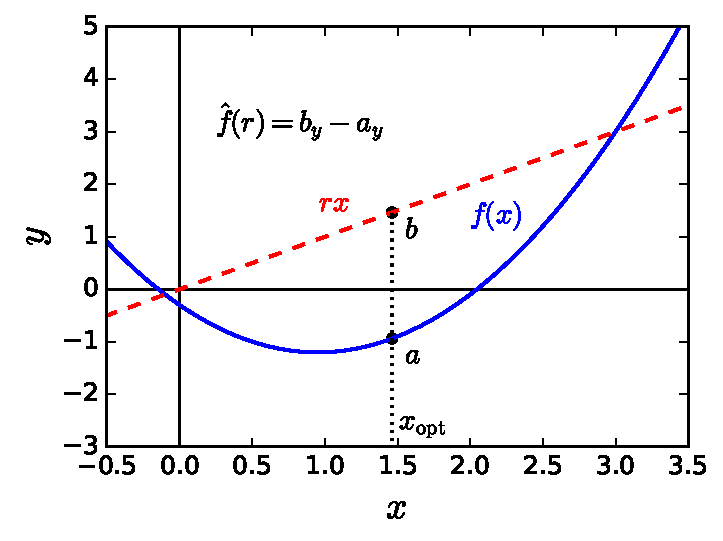
\includegraphics[scale=.65]{img/plots/LT_legendre.pdf}
  \caption{Graphical representation of the Legendre transform. (blue-line) Convex function, $f(x)=x^2-1.9x-0.3$, to be transformed. (red-dashed) Constant slope line passing by the coordinate system origin, $rx$. The Legendre transform is the maximal difference between $rx$ and $f(x)$ at the same $x$. In this case, the vertical distance between $a$ and $b$.}
  \label{fig:lt-geometric-legendre}
\end{figure}

The inverse transformation is simply obtained by applying again the same technique.
One fully recovers the
\be
  f(x) = \max_{r}\{rx-\hat{f}(r)\}.
\ee

Let us develop the example shown in the Figure~\ref{fig:lt-geometric-legendre}, where the function is $f(x)=x^2-1.9x-0.3$.
In this case the problem is well defined on the complete real axis.
Now, one has to find the maximum of $g(r,x)=rx-f(x)$ for all $\forall r$.
This maximum is easily obtained in this particular case with usual techniques.
On has to solve for x the following equation $\partial_x g(r,x) = 0$. Thus, the maximum is at $x_{\text{opt}} = \frac{r+1.9}{2}$ and hence, the Legendre transform is the following,
\be
  \hat{f}(r) = \frac{r^2}{4}+0.95r+1.2025.
\ee
If one applies again the transformation the resulting function is again the original one.
